\chapter{Overview of CryptDB}
\label{chp:overview_cryptDB}

This chapter covers the overview of CryptDB, starting with the system architecture, followed by its different encryption mechanisms and encryption layer adjustments. Along with the investigation, a small application will be introduced and used as an example to help the reader in understanding the practical and impractical usages of CryptDB.

\section{System Architecture}

CryptDB's architecture (Figure \ref{cryptdb_plain}) is divided into two pieces, a proxy server and a database server. The proxy server is an intermediate server placed between the application server (used by the application to manage key set-up and interacting with clients) and the database server. The proxy server's purpose is to intercept queries going from the application to the database and anonymize the information of the query, as well as decrypting results going from the database server to the user's application. By doing so, it eliminates the possibility of eavesdropping attackers to obtain any sensible information. %Kommentere at Microsoft hevder å ha brukt freq attack her.

\begin{figure}[H]
	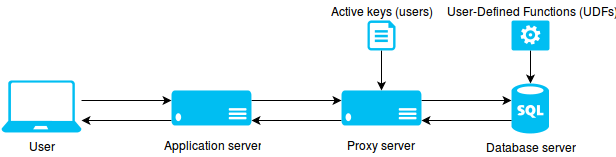
\includegraphics[scale=0.6]{CryptDB_Plain.png}
	\caption{System architecture of CryptDB interacting with a client application}
	\label{cryptdb_plain}
\end{figure}

Another vital part of the proxy server's domain is to issue queries to the database that adjusts the encryption layer (or onion layer) of the data items(s) that the user has issued a query on, which will be discussed in section \ref{adjust_enc_level}. The last responsibility of the proxy server is to keep track of the users that are currently logged in using a table of active keys. In addition to keeping the list of active keys, the proxy server also keeps an embedded database with the schemes of the encrypted tables in the database. By storing this, the proxy server keeps a continuous picture of the encryption layer for each column, which is used for adjusting the encryption level (or layer) for a column in order to allow certain types of functionality.

The authors \citep{CryptDB_Main_Paper} have implemented CryptDB both with MySQL and PostgreSQL database management systems. CryptDB requires no modifying of the database system, other than adding a set of \Gls{udf}. \Gls{udf} in CryptDB allows the database to perform cryptographic operations on the encrypted data, as well as adjust the encryption level of different columns.

CryptDB has two operational modes, or principals. One for applications consisting of only one user, and another for multi-user applications. Application keys consists of both a symmetric key rooted in the users application password and a public-key pair. When logging in, the proxy derives encryption keys with the user's password as the root. These keys are used for accessing the data items that are accessible to that particular user and to encrypt new items. When the user logs out, the keys are deleted from the proxy server.

\subsection{Single-user Mode}
If an application is created with a single user in mind, then it should be running in the single-user mode where the keys are derived from one secret master key which is rooted in the user's password. By running in this particular mode, the user has access to all data encrypted through the proxy server. When running is this mode, the proxy server and the application are considered to be trusted. The database server however, is considered to be untrusted and subject to the snooping of a curious database administrator owning the server system hosting the database. As of the most recent versions of the CryptDB software, only the single-user mode is supported, which has been used to create a small demo application described in Chapter \ref{chp:software}.

\subsection{Multi-user Mode}
Picture a simple online discussion forum, where users can interact by posting messages to discussion boards or sending each other private messages. As described in Section \ref{chp:database_Security}, database applications are in need of access control in order to restrict access to certain tables based on the user's credentials, hence the need for declaring user entities as well as different groups. But how can a user read messages on the discussion board if they are encrypted by another user's key? What about private messages, with suffers from the same case, as they will be encrypted with the sender's key? CryptDB solves these cases by letting developers use annotations in their schemas.

Table \ref{annotations} shows a basic use of such annotations. \verb!PRINCTYPE! is used to annotate external users, which are authenticated through the access control by providing their password, and internal users, which are entities inside the database. \verb!ENC_FOR! is used to indicate which columns that consist sensitive data, and in the next column CryptDB needs to store which principals that should have access to the sensitive column. Okay, so we have access to the column, but how can we decrypt something encrypted with someone else's keys?

\begin{table}[H]
\begin{Verbatim}[frame=single]
PRINCTYPE physical_user EXTERNAL;
PRINCTYPE user, msg;

CREATE TABLE privmsgs (
	msgid integer,
	subject varchar(255)	ENC_FOR (msgid msg),
	msgtext text		ENC_FOR (msgid msg) );

CREATE TABLE privmsgs_to (
	msgid integer,
	recvid integer,
	sendid integer,
	(sendid user) SPEAKS_FOR (msgid msg),
	(recvid user) SPEAKS_FOR (msgid msg) ); 
\end{Verbatim}
\caption{Use of policy annotations when creating multi-user applications}
\label{annotations}
\end{table}
CryptDB chains encryption keys used to encrypt columns or data items to the root key, which is the user's password. The \verb!SPEAKS_FOR! annotation gives a principal access to all the keys that the principal it speaks for has access to. For example in Table \ref{annotations}, both the user sending the private message and the user receiving it, speaks for the principal type \verb!msg! and thereby has access to all the keys of the \verb!msg! entity. This basically means that the secret key of the message is encrypted two times, one time with the sender's key and one time with the receiver's key.

Consider this case: Alice wants to send a private message to Bob, which means that the private message needs to be encrypted two times using both Alice and Bob's secret keys. Keys of users who are logged in are kept in a table at the proxy server, but what happens when the proxy server needs to encrypt something with a key which at the time is inaccessible? The keys that are used by a principal to encrypt consists of both a symmetric key and a public-private-key pair. When both parties are logged in, the proxy uses their symmetric keys to encrypt the message. If Bob is currently logged out, it encrypts the message using his public key so that he can decrypt it using the corresponding private key when he logs in.

As previously mentioned, the current version of CryptDB has only the option of developing single-mode applications. One may react to the fact that the developers has stopped maintaining such a regular and useful way of developing applications with multiple user's and interaction between users. However, Mylar \cite{mylar_homepage} creators of CryptDB's new project. Mylar addresses the threat of when the insecure proxy server is compromised by an attacker, and how to protect the data of the users in such events. During a proxy server in CryptDB, the only parties that are compromised are those who are currently logged in, where their keys are stored in the table at the proxy server.

\section{SQL-Aware Encryption and the Onion Scheme}

CryptDB uses an encryption scheme called \emph{SQL-aware encryption} or \textit{onion encryption}. Basically, this is a collection of different encryption schemes, each providing different levels of security and computations to be executed. Data items stored using CryptDB are encrypted multiple times using these different schemes, or layers, of encryption. The result is a onion-like structure where the outer layers provide maximum security and low functionality, while the inner layers provide less security, but more functionality.

As a scenario in order to describe the different operations and situations in CryptDB, assume a simple employee application with a table structure and some example records as shown in Table \ref{demoapp_table}. Our application is created in order to provide some insight in the salary distribution within our firm, with respect to age, number of years within the firm and employment division. EmplNum is the number associated with the employee in other systems and applications, and SSN is the Social Security Number of the employee used for creating pay checks and similar operations.

\begin{table}[H]
\centering
\begin{tabular}{| r | r | l | r | r | r | l |}
\hline
  Id & EmplNum & Name & SSN & Age & Salary & Division \\
  int & int & varchar(255) & varchar(255) & int & int & varchar(255) \\
 \hline \hline
 1 & 42 & Alice & 24127312345 & 42 & 440000 & Marketing \\
 2 & 1 & Bob & 17054623456 & 69 & 850000 & Management \\
 3 & 1337 & Charlie & 31129134567 & 23 & 390000 & Engineering \\
 4 & 123 & Donna & 11117945678 & 36 & 510000 & Management \\
 \hline

\end{tabular}
\caption{Employee table for a simple employee application with example records}
\label{demoapp_table}
\end{table}


\subsection{Random}
\Gls{random_onion} is the highest security level in CryptDB and provides the maximum security found in encryption scheme. It uses a strong block cipher such as Blowfish or \Gls{aes} in \Gls{cbc_mode} mode and a random initialization vector (IV) to ensure that the block cipher is probabilistic \citep{CryptDB_Main_Paper}. \Gls{random_onion}, being the maximum security level provided, does not allow any computation to be done on the encrypted data. In other terms, this level is a natural choice for sensitive data that are only meant to be read. When a block cipher is probabilistic, it has properties such that when encrypting the same message $m_1$ multiple times, the resulting ciphertexts are unequal. 

For example, given two encryptions of the same plaintext $c_1 = E_k(m_1)$ and $c_2 = E_k(m_1)$, the resulting ciphertexts are $c_1$ and $c_2$ such that $c_1 \neq c_2$. Operations supported by this scheme are \verb!SELECT!, \verb!UPDATE!, \verb!DELETE! and \verb!INSERT!. It also supports altering an existing table by removing or adding columns using the \verb!ALTER! statement. In our sample application, the SSN would be the most natural thing to stay encrypted under \gls{random_onion} at all times, as there are not many natural operation to perform on such numbers. However, the other columns are not likely to be encrypted under \gls{random_onion} as it is likely that the application would want to perform some operations which demands a lower encryption level. As for an example, take the perhaps most natural query at this encryption level, the \verb!INSERT! statement

\begin{verbatim}
INSERT INTO employee_table
VALUES('', 5, 'Eric', '29026056789', 55, 680000, 'Engineering');
\end{verbatim}

\noindent
which adds a record in the database containing Eric's information. When it comes to \verb!SELECT!, \verb!DELETE! and \verb!UPDATE!, it only supports regular queries without the \verb!WHERE! clauses and similar statements:

\begin{verbatim}
SELECT * FROM employee_table;

UPDATE employee_table SET salary = 0;

DELETE FROM employee_table;
\end{verbatim}


\subsection{Deterministic}
Where \Gls{random_onion} allows no computation to be done on the encrypted data, the next layer does. \Gls{deterministic_onion} is an encryption scheme enabling the application to perform standard SQL operations such as equality checks, distinct, group by and count. By allowing these sorts of computation, the application leaks information to an adversary. In particular, it leaks which ciphertexts that decrypts to the same plaintext value. Following the previous example; if the scheme encrypted the message $m_1$ two times, the resulting ciphertexts $c_1$ and $c_2$ are such that $c_1 = c_2$. For our sample application, \Gls{deterministic_onion} would be the scheme used when allowing operations such as \verb!GROUP BY!, \verb!DISTINCT! and \verb!COUNT!. Continuing with our sample application, we now want to find out what types of departments that exists in our table

\begin{verbatim}
SELECT DISTINCT Division
FROM employee_table;
\end{verbatim}
\noindent
which returns \verb!'Engineering'!, \verb!'Marketing'! and \verb!'Management'!. As described, a deterministic scheme encrypts the same plaintext to the same ciphertext every time. By taking advantage of this, CryptDB is capable of iterating over the encrypted data and return a distinct selection of the different ciphertexts observed. At the \gls{deterministic_onion} layer the \verb!WHERE! clause is also supported when running equality checks. An example usage is the query below, where the name, age and salary of all employees from the management division are returned

\begin{verbatim}
SELECT Name, Age, Salary
FROM employee_table
WHERE Division = 'Management';
\end{verbatim}

For the encryption, DET uses a strong block ciphers, and either with 64-bit or 128-bit block size. If a value is larger than 128-bits, it leaks  prefix equality when used with AES \citep{CryptDB_Main_Paper}. In order to cope with leaking prefix equality, the authors have designed their own version of the CMC mode.


\subsection{Order-Preserving Encoding}

Since \Gls{sql} also allows the user to compute on order relations between items, CryptDB introduces an \Gls{ope_onion} scheme \citep{CryptDB_Main_Paper}. This scheme is based on a requirement where the sort order of the ciphertext matches the sort-order of the corresponding decrypted plaintexts. It also requires that the scheme reveals no other information about the plaintexts, other than the respective order. This common operation in \Gls{sql} supports order comparison, which can be used for range checks, ranking, sorting, and extracting minimum and maximum values. 

CryptDB uses a modified version the scheme proposed by Boldyreva et. al \citep{ope_cryptdb} as their OPE scheme, which is a random order-preserving injective function. An injective function is a one-to-one random mapping function that preserves the order of the elements. It uses a Hyper Geometric Distribution (HGD), and uses a lazily sampling to generate ciphertext elements from the set on demand.


Popa et al. has also proposed 

DETTE SKAL JEG SKRIVE SØNDAG


% Has not been implemented in CryptDB yet because of other priorities. CryptDB uses \cite{ope_cryptdb} for their OPE scheme. Random order-preserving injective function
% the hypergeometric (HG) and negative hypergeometric (NHG) probability distributions
% Uses a Hypergeometric Distribution.

% Lazy, so it is not need to generate the whole range, but rather just an element when necessary. Lazy generates in range a->b with respective inverse

%Popa et al. \cite{CryptDB_OPE_Encoding} introduces a scheme called \Gls{mOPE} where the main technique is mutable ciphertexts. Mutability (or malleability) is a cryptographic property allowing the transformation of one ciphertext into another. More formally, given a plaintext $m_1$, it is possible to transform it into a valid encryption $f(m_1)$ by using a valid function $f$ without further knowledge of $m_1$.
%
%\Gls{mOPE} uses a balanced binary tree for searching which contains encryptions of all the plaintext's values and a table of \Gls{ope_onion} encodings where the encoded value of a ciphertext is its path from the root to the particular node in the binary tree. If $y$ is greater than $x$, then $y$ will be located to the right of $x$ in the tree. It also uses an interactive protocol when inserting a value into the search tree, where the server and the client plays a query game. The client asks for the encrypted root node, decrypts it and determines whether the value to be inserted is smaller or larger than the root. It replies to the server with a $0$ or $1$, making the server traverse the tree to the left or right and replying with the next encrypted node. This little game continues until there are no child nodes. In order to avoid the tree being too deep, \Gls{mOPE} uses a tree-balancing transformation summary which describes operations (most of them split-and-merge operations) that are completely done by the server.
%
%The balancing procedure ensures that the height of the tree is bounded by $\log(N)$, where $N$ is the number of encrypted values. Because both client and server needs a shared understanding of the structure of the search tree, the client computes a Merkle hash of the root of the tree. A Merkle tree is a tree where every parent node is labelled with the hash of all of its children's labels \cite{Merkle}. By performing the Merkle hash, the client is able to check whether the server behaves maliciously or not (Malicious in this setting would be if the server performed other operations than the client requested) by comparing its own Merkle hash of the root with the one delivered by the server.


The OPE layer is the encryption layer that adds the most functionality
When searching for the persons in our imaginary firm that has a yearly salary over 500 000, the query uses the \verb!WHERE! clause and then performs an order check where it navigates down the binary three for items that has a salary larger than the requested value.

\begin{verbatim}
SELECT Name, Salary
FROM employee_table
WHERE Salary > 500000;
\end{verbatim}


\subsection{Homomorphic Encryption}
Another vital part of \Gls{sql} is the ability to perform addition and multiplication. For CryptDB to be able to perform these operations, it utilizes a \Gls{hom_onion} scheme. As previously described, homomorphic encryption is a technique that enables computation on encrypted data without decrypting it first. CryptDB uses Pailler multiplication \cite{Paillier} for enabling summation operations. If our application is in need for finding out the total sum of the salaries within the firm, we do something like this

\begin{verbatim}
SELECT SUM(Salary)
FROM employee_table;
\end{verbatim}

\noindent
Or extracting the total salary for each division by using the \verb!GROUP BY! clause

\begin{verbatim}
SELECT Division, SUM(Salary)
FROM employee_table
GROUP BY Division;
\end{verbatim}

Multiplication was not initially implemented, but has been implemented in some versions of CryptDB by an outside team using the El Gamal cryptosystem \cite{cryptdb_guidelines}. 


\subsection{Equality Join and Order-Preserving Join}
When it comes to joining columns, two cases are supported in CryptDB. The first is the regular equality join (EQ-JOIN) between two columns, and the other is range joins (OPE-JOIN) which involves order relation checks. Ideally, the proxy server should know in advance which columns that should be allowed to be joined in order to encrypt these column with the same key. Because of the key-chaining approach where each data item is encrypted with a new key, CryptDB is in need of a separate encryption scheme in order to compute joins in a safe manner.

The authors \citep{CryptDB_Main_Paper} introduces a new cryptographic primitive for equality joins, \gls{join_adj}, which is a deterministic function. The idea is to let the proxy server adjust the encryption keys of columns in real-time, based on the observed query. By using this approach, CryptDB avoids the database server to compute joins on its own as attempt to learn about relations between different columns. When a join query is observed at the proxy, it sends an adjusted key to the database server enabling it to adjust the values in one of the two affected columns. When an adjustment has been done, the columns share the key until the proxy server issues a new adjustment key to either one of the columns.

The second case is the order-preserving join, which depends on the \gls{ope_onion} scheme previously described. The binary tree structure of the scheme makes in infeasible to use the same approach as EQ-JOIN. Therefore, CryptDB has a requirement that columns where such joins is applicable have to be declared by the application in beforehand and encrypted under the same key. If this measure has not been addressed, CryptDB will simply encrypt all columns with the same key.


Example here: join on empl\_num

\subsection{Search}
In order to perform search for words in the encrypted texts, CryptDB has a scheme called SEARCH. This was an implementation of the cryptographic protocol suggested by Song et al. making it almost as secure as the \gls{random_onion} scheme \citep{CryptDB_Main_Paper}. The main idea is to split a text encrypted with SEARCH into individual keywords on a given delimiter specified by the application developer. Removal of duplicate keywords and randomly permute them are also added to enhance the security. When executing a search, the server would be given an encrypted token of the keyword, and would retrieve encrypted values matching the token. Originally, SEARCH could perform \texttt{LIKE} operations as other database systems, but in the most recent version of CryptDB's software it has been deprecated. 

\subsection{Wrapping the Layers}

These different layers are wrapped into four different classes or \emph{onions}, namely \texttt{EQ}(Equality checks), \texttt{ORD}(Order relations), \texttt{SEARCH}(Searching) and \texttt{ADD}(Addition) as shown in Figure \ref{cryptdb_onions}. Each onion has a special purpose in means of supporting certain operations, and every data item is encrypted each of the different onions using the different layers. However, the application does not necessary maintain all of onions. There is, for example, no need for maintaining the ADD-onion if the data item is a string.

\begin{figure}[H]
	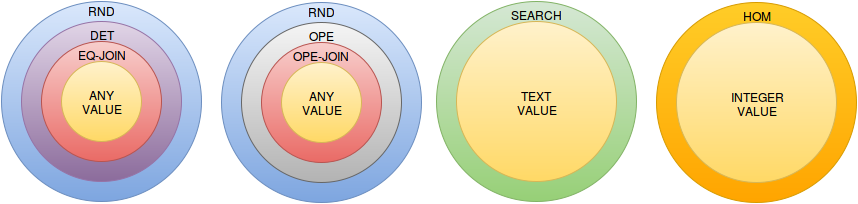
\includegraphics[scale=0.42]{Onions.png}
	\caption{Overview of the structure of the SQL-aware Encryption Scheme. From left: The EQ-onion, ORD-onion, SEARCH-onion and ADD-onion}
	\label{cryptdb_onions}
\end{figure}


\section{Adjusting the Encryption Level Based on the Query}
\label{adjust_enc_level}

Okay, so there is an encapsulation of different encryptions for each data item, and our ideal scenario is that our data is encrypted at the highest, feasible level at all times.  But how is the system supposed to perform a range check if the utmost layer is the \gls{random_onion} which does not support any functionality at all?

CryptDB solves this particular case gracefully by having the proxy server observe incoming queries in real-time. After observing a query, it checks its embedded table holding the encryption level of the all columns whether or not the current encryption level of the inflicted columns are supporting the query. For example in our sample application, the user has issued the query 
\begin{verbatim}
SELECT *
	FROM employee_table
	WHERE salary > 5000000;
\end{verbatim}

Have in mind that all data items at this point is encrypted with \gls{random_onion} as the utmost layer. What the proxy does, is that before sending the rewritten query to the database server, it sends an \verb!UPDATE! query first. This query orders the database server to remove the outer encryption level of the ORD-onion to match the \gls{ope_onion} layer, before it sends the rewritten query. Figure \ref{ope_layer_adjustment} illustrates how the proxy server observes the query, and issues the \verb!UPDATE!. \verb!SET! is used to change the current encryption level of the ORD-onion, and \verb!cryptdb_decrypt_int_sem! is the name of the UDF that the server will use to adjust the encryption layer to  support the query. The curious string \verb!'???]???G??+?,?#'! is the encrypted key which the server will use along with the UDF.

\begin{figure}[h]
	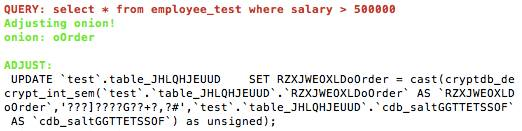
\includegraphics[scale=0.7]{terminal/adjustOnionLayer.jpg}
	\caption{Encryption layer adjustment performed by proxy server upon receiving a query. (Is the figure too small/hard to read?. Adjust colors?)}
	\label{ope_layer_adjustment}
\end{figure}

\newpage
After performing the encryption layer adjustment, the proxy rewrites the query as shown in Figure \ref{rewritten_query}. As described, each of the columns are anonymized upon the creation of a table. The proxy server keeps table schemes in order to substitute the different parts of the query so it matches the encrypted columns in the database. For the record, 'test' is the name of the current database.  

\begin{figure}[h]
	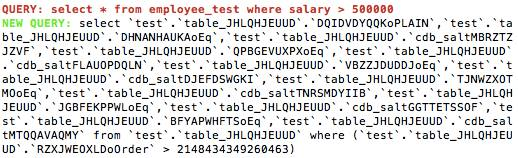
\includegraphics[scale=0.7]{terminal/executeQuery.jpg}
	\caption{Rewritten query to be sent to server after encryption level adjustment. (Is the figure too small/hard to read?. Adjust colors?)}
	\label{rewritten_query}
\end{figure}


\section{Security}

Overview of the security aspects of CryptDB

\section{Limitations}


\gls{fhe} is nowhere near being practical yet, but CryptDB tries it best to be a somewhat practical \gls{he} scheme allowing a set of operations that they claim to be enough to support 99.5\% of all queries observed in a \gls{sql} trace from a production MySQL server \citep{CryptDB_Main_Paper}. 

Data structures that are not supported:

Float, Double, Timestamp, Date, Time, DateTime, Year, Newdate, Bit, Enum, Set, Geometry

Nested queries

On the hack queries and other things that simply does not work with CryptDB. 